% die Standard-Dokumentenklasse
\documentclass[11pt,a4paper]{article} %% 1.Ebene = chapter, headings

% input encoding, font encoding, outline font
\usepackage[utf8]{inputenc} 
\usepackage[T1]{fontenc} 
\usepackage{lmodern}
\usepackage{tcolorbox}
% Sprache
\usepackage[german]{babel}
\usepackage[section]{placeins}

% Absatzformatierung
\setlength{\parindent}{0pt}
\setlength{\parskip}{1ex plus 0.5ex minus 0.5ex}

% erweiterte mathematische Symbole
\usepackage{amsmath} 

% für Abbildungen
\usepackage{graphicx} 

% für Tabellen
\usepackage{booktabs}

% für Hyperlinks
\usepackage[colorlinks]{hyperref}
\graphicspath{}




\begin{document}

{
	\centering 
	\large 
	Physiklabor für Anfänger*innen \\
	Ferienpraktikum im Sommersemester 2018 \\[4mm]
	\textbf{\LARGE 
		Versuch 36: Der Adiabatenexponent
	} \\[3mm]
	(durchgeführt am 14.09.2018 bei Nico Strauß) \\
	Ye Joon Kim, Marouan Zouari\\
	\today \\[10mm]
}

\section{Einleitung}
Die Wärmekapazität von einem bestimmten Material ist nicht immer Konstant und hängt von der Art ihrer Zustandsänderung ab. Die Wärmekapazität bei einer isochoren Zustandsänderung, $c_V$, und bei einer isobaren Zustandsänderung, $c_p$, unterscheiden sich im Idealfall mit einem Faktor von $R$, die universelle Gaskonstante. Das Verhältnis von $c_V$ und $c_p$, $\kappa$, heißt der Adiabatenexponent, und taucht auch in der Poisson'schen Gleichung 
$$pV^\kappa = \textrm{const.  (Für Adiabatische Zustandsänderungen)}$$ 
auf. Deswegen der Name ,,Adiabatenexponent''

\section{Ziel des Versuchs}
Das Ziel dieses Versuchs ist es, die Adibatenexponente von Luft und Argon mit einem Rüchardt-Flammerfeld-Aufbau zu bestimmen. 

\section{Durchführung}
Siehe Abbildungen im Kapitel Aufbau für die Bauteile. 

Zur Bestimmung der Adiabatexponenten wurde einen Rüchardt-Falmmerfeld-Aufbau benutzt (Siehe Abbildung 1). Die Zweiwegehähne wurden zuerst so umgestellt, sodass der Luft von dem Behälter in den Kolben fließen kann. Das Auslassventil wurde dann für eine Minute geöffnet, um den Apparat zu spülen. Dann wurde das Feinventil gedreht, bis der Schwingkörper anfing, zu schwingen. Das Zählgerät wurde aktiviert, bis das Gerät genug Schwingungen (100 oder 200 Schwingungen) detektiert hatte. Die Anzahl Schwingungen und die Zeit wurden dann aufgenommen. Dieses Messverfahren wurde fünfmal wiederholt.

Die Zweiwegehahn wurde dann zu umgestellt, sodass Argon dadurch fließen kann. Das Auslassventil wurde für fünf Minuten geöffnet, um den Apparat zu spülen. Danach wurde das Messverfahren, wie in oben erläutert, durchgeführt und Daten aufgenommen. 
\section{Aufbau}
Der Rüchartdt-Flammerfeld-Aufbau besteht aus die folgenden Bauteilen.
\\\ 
\textbf{Der Induktive Signalabnehmer} wird zur Zählung der Anzahl Schwingungen benutzt. 
\\\
\textbf{Das Glaskolben} behaltet die Druckluft, die durch das Loch an dem Glasrohr teilweise ausfließt, damit eine Schwingung erzeugt wird
\begin{figure} [h]
\centering
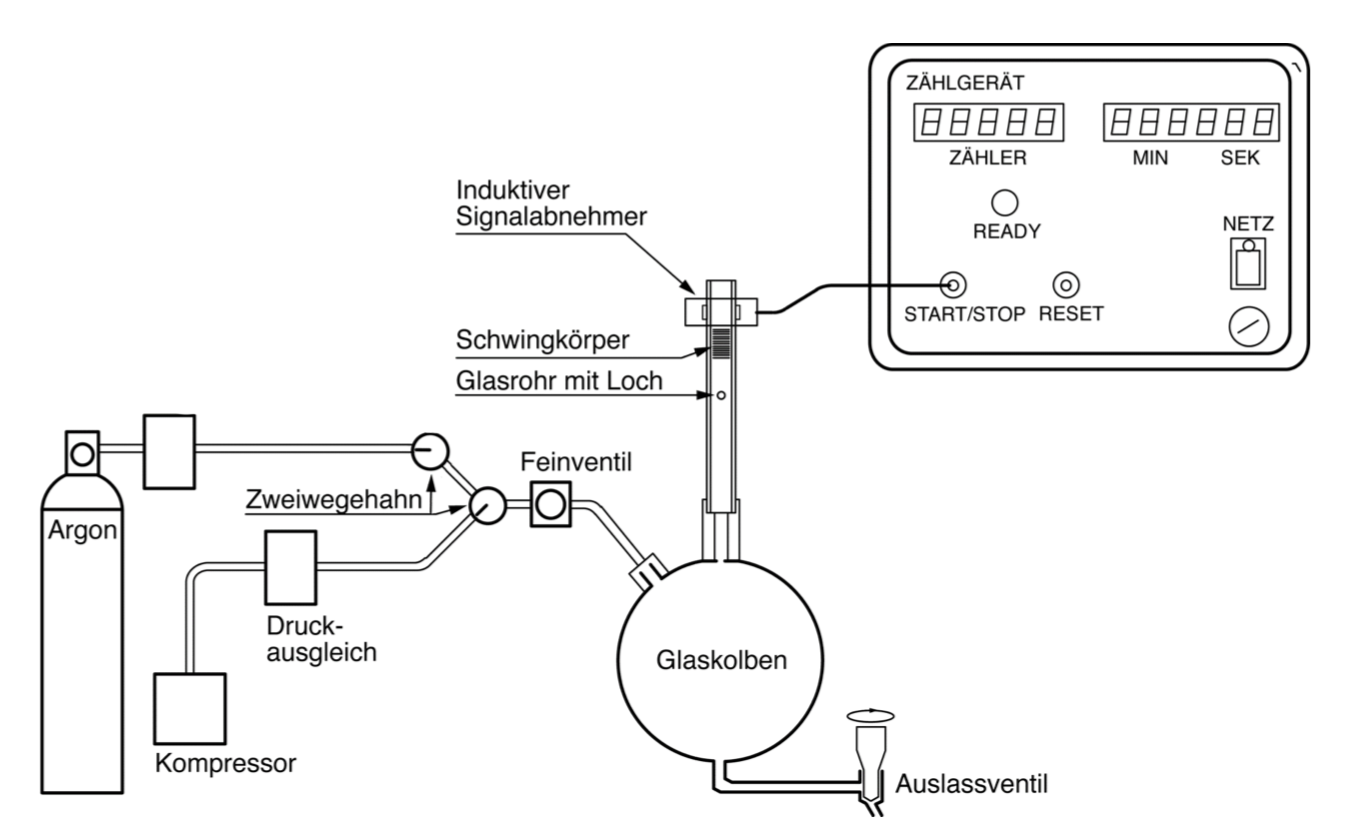
\includegraphics[width=\linewidth]{Abb1}
\caption{Versuchsaufbau. Ein Rüchartdt-Flammerfeld-Aufbau. ("Versuchsanleitungen")}
\end{figure}

\section{Auswertung und Fehleranalyse}
Siehe Anhang für rohe Daten.

Zur Berechnung der Adiabatenexponent wird die folgenden Formel benutzt:

\begin{equation}
\kappa = \frac{4\pi^2 m V}{A^2 p T_S^2}
\end{equation}
mit:
$$ A = \frac{\pi d^2}{4} $$
$$ p = p_A + \frac{mg}{A} $$
wobei:

\begin{itemize}
	\item $m$ die Masse des Schwingkörpers
	\item $V$ das Volumen des Schwingkörpers
	\item $A$ die Querschnittsfläche des Schwingkörpers
	\item $p$ der mittlere Druck des Gases im Kolben
	\item $T_S$ die Schwingungsdauer
	\item $d$ der Durchmesser des Schwingkörpers
	\item $p_A$ der äußere Luftdruck 
\end{itemize}



\subsection{Der Adiabatenexponent von Luft}
Um $T_S$ zu bestimmen wurden die totalen Messzeiten durch die Anzahl Schwingungen geteilt. Die dadurch berechnete Mittelwerte sind:
\begin{table} [h]
	\begin{tabular*}{0.99\textwidth}{@{\extracolsep{\fill}}cccccc}
		\toprule
		Messreihe & $T_S$ & $\Delta T_S$  \\
		& s & s   \\
		\bottomrule
		1 & 0,393 & 0,004 \\
		2 & 0,391 & 0,004 \\
		3 & 0,387 &  0,008\\
		4 & 0,392 & 0,003 \\
		5 & 0,392  & 0,004 \\
		\bottomrule
	\end{tabular*}
	\caption{Die Werte für $T_S$, die mittlere Schwingdauer, und deren Unsicherheiten.}
\end{table} 

\begin{tcolorbox}[colback=white]
\subsubsection{Beispielrechnungen}
Für die Unsicherheiten von $T_S$ wurde die folgende Formel für die Unsicherheit des Mittelwerts benutzt:
$$\Delta T_S = \frac{\Delta T}{\sqrt{n}}$$
Wobei $T$ für die gesamte gemessene Zeitdauer steht. 





\end{tcolorbox}


und dadurch lassen sich die Werte für $\kappa$ berechnen:

\begin{table} [h]
	\begin{tabular*}{0.99\textwidth}{@{\extracolsep{\fill}}cccccc}
		\toprule
		Messreihe & $\kappa$ & $\Delta \kappa$  \\
		\bottomrule
		1 & 1,404 & 0,020 \\
		2 & 1,415 & 0,020 \\
		3 & 1,442 &  0,040 \\
		4 & 1,407 & 0,020 \\
		5 & 1,412  & 0,020 \\
		\bottomrule
	\end{tabular*}
	\caption{Werte für die berechneten Adiabatenexponenten und deren Unsicherheiten.}
\end{table} 

\begin{tcolorbox}[colback=white]
\subsection{Beispielrechnungen}
Zur Erleichterung der Berechnungen wurden zuerst die Werte für $A$, $p$ und deren Unsicherheiten berechnet. 

Die Unsicherheiten von $A$ lassen sich mit der vereinfachten Formel für Produkte und Quotienten bestimmen:
\begin{equation}
\vert\frac{\Delta z}{z_0}\vert = \sqrt{(a\frac{\Delta x}{x_0})^2+(b\frac{\Delta y}{y_0})^2} \; \; \textrm{für} z=x^a\cdot y^b. 
\end{equation}
und deshalb ist
$$ A = (1,517 \pm 0,001) \cdot 10^{-4} \textrm{m}^3$$
Für $p$ wurden zuerst die Unsicherheiten von $p_S$ mit der obigen Formel berechnet und danach mit der Formel für Summen berechnet, nämlich:
\begin{equation}
\Delta z = \sqrt{(a\Delta x)^2 + (b \Delta y)^2 ...} \textrm{  für } z = ax+by \dots
\end{equation}

Und endlich können die Unsicherheiten für $\kappa$ mit der Formel (2) berechnet werden. Aber da die Beträge von $\frac{\Delta V}{V}$ und $\frac{\Delta T_S}{T_S}$ überwiegend größer waren als die Beträge der anderen Terme, wurden nur diese zwei Terme berücksichtigt. 

Die Unsicherheit von $\kappa$ lässt sich deshalb schreiben als:
$$ \Delta \kappa  = \kappa \sqrt{(\frac{\Delta V}{V})^2 + (2\frac{\Delta T_S}{T_S})} $$
\end{tcolorbox}

Der Mittelwert und seine Standardunsicherheit lauten:
$$\kappa =  1,412 \pm 0,015$$

\subsection{Der Adiabatenexponent von Argon}

Für die Bestimmung des Adiabatenexponents wurde dasselbe Verfahren in dem ersten Teil benutzt. 

\begin{table} [h]
	\begin{tabular*}{0.99\textwidth}{@{\extracolsep{\fill}}cccccc}
		\toprule
		Messreihe & $T_S$ & $\Delta T_S$  \\
		& s & s   \\
		\bottomrule
		1 & 0,3696 & 0,001 \\
		2 & 0,3686 & 0,001 \\
		3 & 0,3649 &  0,04\\
		4 & 0,3669 & 0,002 \\
		5 & 0,3669  & 0,002 \\
		\bottomrule
	\end{tabular*}
	\caption{Die Werte für $T_S$, die mittlere Schwingdauer, und deren Unsicherheiten.(Für Argon)}
\end{table} 

\begin{table} [h]
	\begin{tabular*}{0.99\textwidth}{@{\extracolsep{\fill}}cccccc}
		\toprule
		Messreihe & $\kappa$ & $\Delta \kappa$  \\
		\bottomrule
		1 & 1,585 & 0,010 \\
		2 & 1,593 & 0,010 \\
		3 & 1,625 &  0,024 \\
		4 & 1,609 & 0,016 \\
		5 & 1,609  & 0,012 \\
		\bottomrule
	\end{tabular*}
	\caption{Werte für die berechneten Adiabatenexponenten und deren Unsicherheiten.(Für Argon)}
\end{table} 

\FloatBarrier
Der Mittelwert und seine Standardunsicherheit lauten:
$$ \kappa = 1,604 \pm 0,016$$

\subsubsection{Systematische Fehler}
Ein möglicher systematischer Fehler ist es, dass es einen Zeitdauer zwischen die Messung der letzten Schwingung und den Stopp der Uhr gibt, da es unmöglich ist, die Messung genau am Ende einer Schwingungsperiode aufzuhören. Deswegen sind die gemessenen Zeiten länger als der Idealfall . Die resultierende Abweichung der gemessenen gesamten Zeit wurde als Maximal 0,4 Sekunde, rund eine Schwingungsperiode, abgeschätzt. Deswegen ist die maximale Abweichung von $T_S$ rund 0,008 Sekunde, was einen Systematischen Fehler von ungefähr 0,06 bei $\kappa$ entspricht. 

\section{Diskussion der Ergebnisse}
Die gemessenen Werte für die Adiabatenexponenten von Luft, $\kappa_L$, und von Argon, $\kappa_{Ar}$ sind:
$$\kappa_L = 1,412 \pm 0,015 \pm 0,060$$
$$\kappa_{Ar} = 1,604 \pm 0,016 \pm 0,060$$

\subsubsection{Vergleich mit den theoretischen Werten}
Luft besteht aus ungefähr 78\% N$_2$ und 21\% O$_2$. Die theoretischen Adiabatenexponenten dieser zwei Gasen lassen sich mit der folgenden Formel bestimmen:
\begin{equation}
\kappa = \frac{3N-b+2}{3N-b}
\end{equation}
Wobei $N$ die Anzahl Atome in dem Molekül und $b$ die Anzahl Bindungen sind. Da N$_2$ und O$_2$ beide zwei Atome und eine Bindung haben (Ohne Berücksichtigung von Mehrfachbindungen), ist der Adiabatenexponent von Luft: 
$$\kappa_L = \frac{7}{5} = 1,4$$

Der Adiabatenexponent von Argon, ein monoatomisches Gas, ist nach Gleichung (4) deshalb:
$$\kappa_{Ar} = \frac{5}{3} \approx 1,67$$

Es ist Offensichtlich, dass der gemessene Werte für den Adiabatenexponent von Luft und Argon mit den theoretischen Werten übereinstimmen, da deren Differenzen  (zwischen die gemessenen und theoretischen Werte) kleiner sind als die Unsicherheiten. 

\subsubsection{Unsicherheiten  und Verbesserungsvorschläge}
Die relativen Unsicherheiten von $\kappa_L$ und $\kappa_{Ar}$ waren:
$$\frac{\kappa_L}{u_{\kappa L}} \approx 0,05$$
$$\frac{\kappa_{Ar}}{u_{\kappa {Ar}}} \approx 0,05$$
, aber das könnte genauer gewesen sein (bis auf $\frac{\kappa}{u_\kappa} \approx 0,01$), gäbe es keine systematische Unsicherheit (Erläutert im letzten Paragraph). Aber im Vergleich mit den anderen Versuchen können die Ergebnisse relativ gut vertraut werden. 

Ein statistischer Fehler war es, dass das Glasrohr am oben offen war, und deshalb könnte das Druckgleichgewicht innerhalb des Rohres von äußeren Faktoren wie z.B der Druckschwankung beeinflusst gewesen sein. Da die Fenster des Zimmers stets offen war, gab es Wind von draußen. Deshalb war der Luftdruck innerhalb des Raumes nicht konstant. Dieses Problem lässt sich lösen, indem man den Raum mehr abgeschlossen macht, wie z.B. die Fenster zu schließen oder die Tür zuzumachen. 

Das im Kapitel 4 erwähnter systematischer Fehler lässt sich lösen, indem man einen anderen Apparat benutzt, der automatisch die Zeitmessung am Start einer Schwingungsperiode startet und am Ende einer Periode stoppt. Dann wäre es möglich eine wesentlich kleinere Unsicherheit bei dem Endergebnis zu haben, da die systematische Unsicherheit rund viermal größer ist als die statistische Unsicherheit. 

\section{Literatur}
,,Versuchsanleitungen zum Physiklabor für Anfänger*innen, Teil 1.''  Albert-Ludwigs-Universität Freiburg: 2018. 
\newpage
\section{Anhang: Rohe Daten}

\begin{table} [h]
	\begin{tabular*}{0.99\textwidth}{@{\extracolsep{\fill}}cccccc}
		\toprule
		Messreihe & $T$ & $\Delta T$ & $n$ & $\Delta$ n  \\
		& s & s & &   \\
		\bottomrule
		1 & 38,87 & 0,1 & 99  & 10\\
		2 & 39,11 & 0,1 & 100 & 10\\
		3 & 19,37 &  0,1 & 50 & 7\\
		4 & 39,22 & 0,1 & 100 & 10\\
		5 & 39,15  & 0,1 & 100 & 10 \\
		\bottomrule
	\end{tabular*}
	\caption{Die Werte für $T$, die gemessene gesamte Zeit, und Anzahl Schwingungen.(Für Wasser)}
\end{table} 
\begin{table} [h]
	\begin{tabular*}{0.99\textwidth}{@{\extracolsep{\fill}}cccccc}
		\toprule
		Messreihe & $T$ & $\Delta T$ & $n$ & $\Delta$ n  \\
		& s & s & &   \\
		\bottomrule
		1 & 92,40 & 0,1 & 250  & 16\\
		2 & 92,15 & 0,1 & 250 & 16\\
		3 & 35,40 &  0,1 & 97 & 10\\
		4 & 55,03 & 0,1 & 150 & 12\\
		5 & 93,37  & 0,1 & 200 & 14 \\
		\bottomrule
	\end{tabular*}
	\caption{Die Werte für $T$, die gemessene gesamte Zeit, und Anzahl Schwingungen.(Für Argon)}
\end{table} 


\end{document}